%%%
 %
 % Copyright (C) 2019 Ángel Iván Gladín García
 %
 % This program is free software: you can redistribute it and/or modify
 % it under the terms of the GNU General Public License as published by
 % the Free Software Foundation, either version 3 of the License, or
 % (at your option) any later version.
 %
 % This program is distributed in the hope that it will be useful,
 % but WITHOUT ANY WARRANTY; without even the implied warranty of
 % MERCHANTABILITY or FITNESS FOR A PARTICULAR PURPOSE.  See the
 % GNU General Public License for more details.
 %
 % You should have received a copy of the GNU General Public License
 % along with this program.  If not, see <http://www.gnu.org/licenses/>.
%%%

%%%%%%%%%%%%%%%%%%%%%%%%%%%%%%%%%%%%%%%%%%%%%%%%%%%%%%%%%%%%%%%%%%%%%%%%%%%%%%%%%%%%%%%%%
\documentclass[letterpaper]{article}
\usepackage[margin=.75in]{geometry}
\usepackage[utf8]{inputenc}
\usepackage[spanish]{babel}
\decimalpoint

\usepackage{listings}
\usepackage{color}
\usepackage{graphicx}
\usepackage{enumerate}
\usepackage{enumitem}
\usepackage{float}

\usepackage{longtable}
\usepackage{hyperref}
\usepackage{commath}

\usepackage{bbm}
\usepackage{dsfont}
\usepackage{mathrsfs}
\usepackage{amsmath,amsthm,amssymb}
\usepackage{mathtools}
\usepackage{longtable}
\usepackage{algorithm}
\usepackage{algorithmic}


%%%%%%%%%%%%%%%%%%%%%%%%%%%%%%%%%%%%%%%%%%%%%%%%%%%%%%%%%%%%%%%%%%%%%%%%%%%%%%%%%%%%%%%%%%%%%%%%5

\usepackage{import}

\usepackage[utf8]{inputenc}

\usepackage{listings}
\usepackage{color}

\definecolor{codegreen}{rgb}{0,0.6,0}
\definecolor{codegray}{rgb}{0.5,0.5,0.5}
\definecolor{codepurple}{rgb}{0.58,0,0.82}
\definecolor{backcolour}{rgb}{0.95,0.95,0.92}

\lstdefinestyle{mystyle}{
    breakatwhitespace=false,         
    breaklines=true,                 
    captionpos=b,                    
    numbers=left
}

\lstset{style=mystyle}
%%%%%%%%%%%%%%%%%%%%%%%%%%%%%%%%%%%%%%%%%%%%%%%%%%%%%%%%%%%%%%%%%%%%%%%%%%%%%%%%%%%%%%%%%


%%%%%%%%%%%%%%%%%%%%%%%%%%%%%%%%%%%%%%%%%%%%%%%%%%%%%%%%%%%%%%%%%%%%%%%%%%%%%%%%%%%%%%%%%
\newcommand{\Z}{\mathbb{Z}}
\newcommand{\N}{\mathbb{N}}
\newcommand{\Q}{\mathbb{Q}}
\newcommand{\R}{\mathbb{R}}
\newcommand{\Pro}{\mathds{P}}
\newcommand{\Oh}{\mathcal{O}} %% Notacion "O"
\newcommand{\lra}{\longrightarrow}
\newcommand{\ra}{\rightarrow}
\newcommand{\ord}{\text{ord}}
\newcommand{\sol}{\textbf{\underline{Solución}: }} %% Solucion
\newcommand{\af}{\textbf{\underline{Afirmación}: }}
\newcommand{\cej}{\textbf{\underline{Contraejemplo}: }}

\usepackage{filecontents}
\begin{filecontents*}{references.bib}
    @book{Hochbaum:1996:AAN:241938,
    editor = {Hochbaum, Dorit S.},
    title = {Approximation Algorithms for NP-hard Problems},
    year = {1997},
    publisher = {PWS Publishing Co.},
    address = {Boston, MA, USA},
    }   

    @misc{Widgerso0:online,
    author = {},
    title = {WidgersonAlgorithm.pdf},
    howpublished = {\url{https://www.ics.uci.edu/~goodrich/teach/graph/notes/WidgersonAlgorithm.pdf}},
    month = {},
    year = {},
    note = {(Accessed on 10/29/2019)}
    }

    @misc{de5fd3ad46:online,
    author = {},
    title = {Fast Approximation Algorithms on Maxcut, k-Coloring
    and k-Color Ordering for VLSI Applications},
    howpublished = {\url{https://pdfs.semanticscholar.org/b4d1/de5fd3ad7e62b1ca1922bb2243d76f08ffe6.pdf}},
    month = {},
    year = {},
    note = {(Accessed on 10/29/2019)}
    }
    
    @misc{VIIIAppr94:online,
    author = {},
    title = {VIII. Approximation Algorithms: MAX-CUT Problem (Outlook)},
    howpublished = {\url{https://www.cl.cam.ac.uk/teaching/1617/AdvAlgo/maxcut.pdf}},
    month = {},
    year = {},
    note = {(Accessed on 10/29/2019)}
    }
\end{filecontents*}

%%%%%%%%%%%%%%%%%%%%%%%%%%%%%%%%%%%%%%%%%%%%%%%%%%%%%%%%%%%%%%%%%%%%%%%%%%%%%%%%%%%%%%%%%

\begin{document}

%%%%%%%%%%%%%%%%%%%%%%%%%%%%%%%%%%%%%%%%%%%%%%%%%%%%%%%%%%%%%%%%%%%%%%%%%%%%%%%%%%%%%%%%%
\title{
        Universidad Nacional Autónoma de México\\
        Facultad de Ciencias\\
        Complejidad Computacional\\
    \vspace{1cm}
    \large
        \textbf{Tarea 5}\\
        \textbf{Algoritmos de aproximación}
}
\author{
    Ángel Iván Gladín García\\
    No. cuenta: 313112470\\
    \texttt{angelgladin@ciencias.unam.mx}
}
\date{29 de octubre 2019}
\maketitle
%%%%%%%%%%%%%%%%%%%%%%%%%%%%%%%%%%%%%%%%%%%%%%%%%%%%%%%%%%%%%%%%%%%%%%%%%%%%%%%%%%%%%%%%%

%%%%%%%%%%%%%%%%%%%%%%%%%%%%%%%%%%%%%%%%%%%%%%%%%%%%%%%%%%%%%%%%%%%%%%%%%%%%%%%%%%%%%%%%%
\newtheorem{theorem}{Teorema}
\newtheorem{example}{Ejemplo}
\newtheorem{corollary}{Corolario}
\newtheorem{lemma}{Lemma}
\newtheorem{definition}{Definicion}
\newtheorem{prop}{Proposicion}


%%%%%%%%%%%%%%%%%%%%%%%%%%%%%%%%%%%%%%%%%%%%%%%%%%%%%%%%%%%%%%%%%%%%%%%%%%%%%%%%%%%%%%%%%
\section{MAX-CUT Problem}
\underline{Definción del problema:} Dada una gráfica no dirigida $G=(V,E)$ la meta es encontrar un
subconjunto $S \subseteq V$ tal que $|E(S, V\setminus S)|$ sea maximizado.

\textbf{MAX-CUT con peso} para cada arista $E \in E$ que tiene un peso no negativo $w(e)$.
Dada una gráfica no dirigida $G=(V,E)$ la meta es encontrar un
subconjunto $S \subseteq V$ tal que $|E(S, V\setminus S)|$ sea maximizado. Maximixar el peso de las
aristas que cruzan en el corte, i.e., maximizar
$w(S) := \sum_{\{ u,v \} \in E(S, V\setminus S)} w(\{ u,v \})$

\begin{figure}[!h]
	\centering
	\begin{minipage}[t]{4cm}
		\centering
		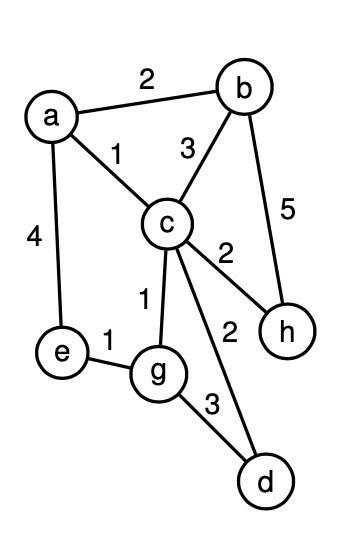
\includegraphics[scale=0.5]{1.png}
	\end{minipage}
	\hspace{3cm}
	\begin{minipage}[t]{4cm}
		\centering
		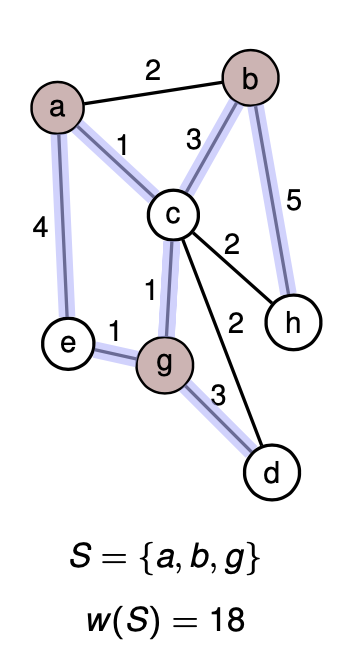
\includegraphics[scale=0.5]{2.png}
	\end{minipage}
\end{figure}

\subsection{Muestreo aleatorio}
Soponer que para cada vértice $v$, escogemos aleatoriamente e independientemente ponemos $v$ en $S$
con probabilidad $1/2$ y en $V \setminus S$ con probabilidad $1/2$. Entonces este algoritmos es un
algoritmo de aleatorio de dos aproximaciones.
\begin{proof}
    Expresamos la esperanza del peso de un corte aleatorio $(S, V \setminus S)$ como:
    \begin{align*}
        E[w(S, V \setminus S)]
            &= E[ \sum_{\{ u,v \} \in E(S, V\setminus S)} w(\{ u,v \}) ]\\
            &= \sum_{\{ u,v \} \in E} Pr[ \{ u \in S \cap c \in (V \setminus S) \} \cup
                \{ u \in (V \setminus S) \cap v \in S \} ] \cdot w(\{ u,v \})\\
            &= \sum_{\{ u,v \} \in E} (\frac{1}{4} + \frac{1}{4}) \cdot w(\{ u,v \})\\
            &= \frac{1}{2} \sum_{\{ u,v \} \in E} w( \{ u,v \} ) \geq \frac{1}{2} w^*.
    \end{align*}
\end{proof}

Búsqueda local
\lstset{language=Pascal}

\begin{algorithm}[H]
    \caption{Búsqueda local $(G,w)$}
    Sea $S$ un conjunto arbitrario de $V$
    \begin{algorithmic}
    \WHILE{flag = 1}
    \STATE{flag = 0}
    \IF{$\exists u \in S$ con $w(S \setminus \{u\}, (V \setminus S) \cup \{u\}) \geq w(S, V\setminus S)$}
    \STATE $S=S \setminus \{u\}$
    \STATE{flag = 1}
    \ENDIF
    \IF{$\exists u \in S$ con $w(S \cup \{u\}, (V \setminus S) \setminus \{u\}) \geq w(S, V\setminus S)$}
    \STATE $S=S \cup \{u\}$
    \STATE{flag = 1}
    \ENDIF
    \ENDWHILE
    \RETURN S
    \end{algorithmic}
\end{algorithm}

\begin{figure}[!h]
	\centering
	\begin{minipage}[t]{4cm}
		\centering
		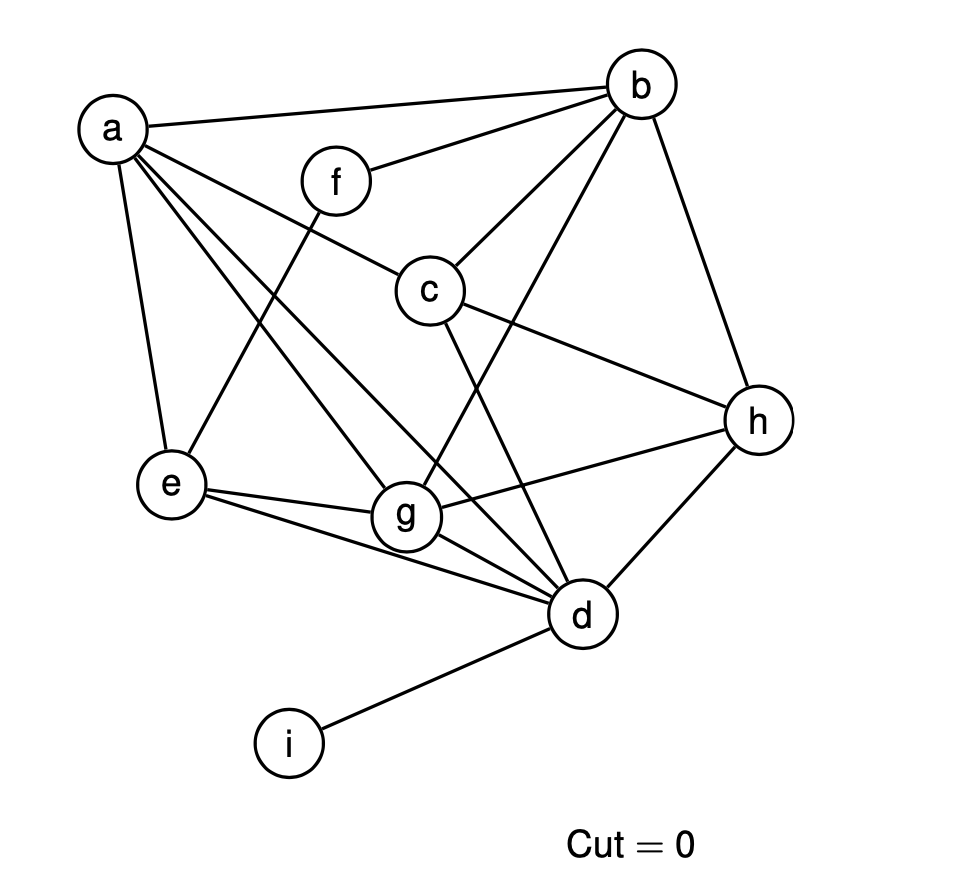
\includegraphics[scale=0.5]{3.png}
	\end{minipage}
	\hspace{3cm}
	\begin{minipage}[t]{4cm}
		\centering
		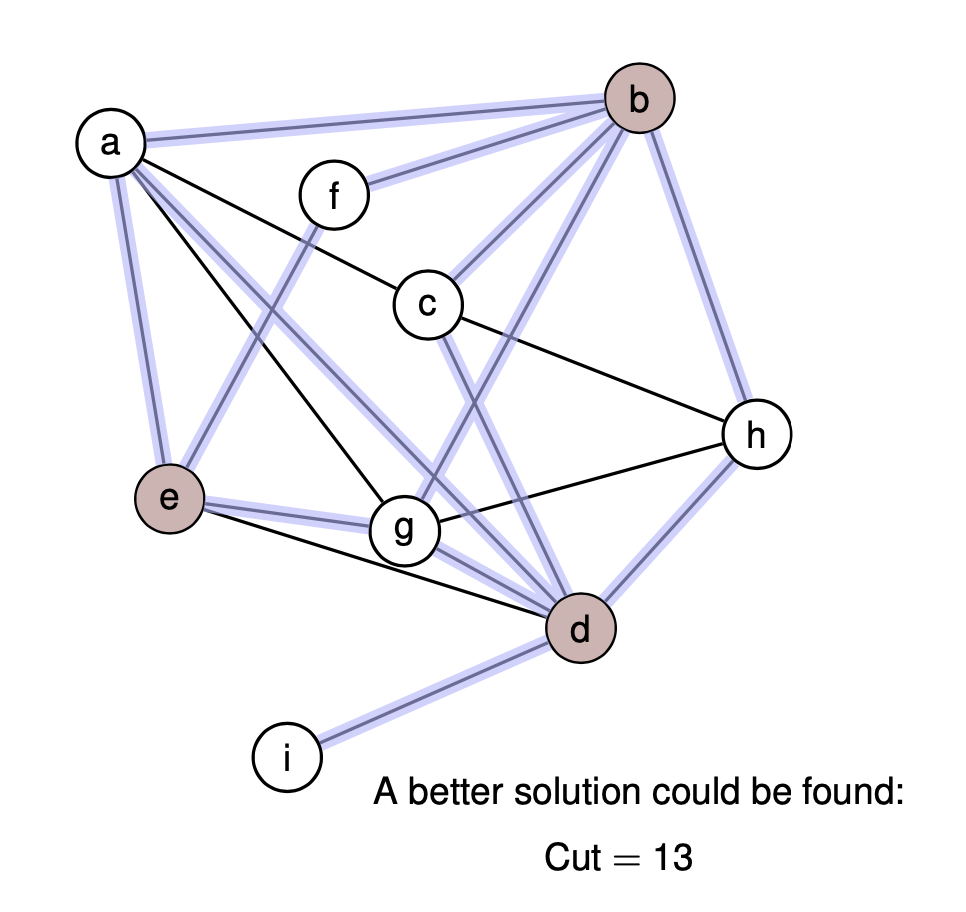
\includegraphics[scale=0.5]{4.png}
	\end{minipage}
\end{figure}

\begin{theorem}
    El corte regresado por la búsqueda local satisface $W \geq (1/2)W^*$.
    \begin{proof}
        En el momento en el que acaba, para cada vértice $u \in S$:
        \[
            \sum_{v \in V \setminus S, v \sim u} w(\{u,v\}) \geq 
            \sum_{v \in S, v \sim u} w(\{u,v\}), \tag{1}
        \]
        Similarmente, para cada vértice $u \in V\setminus S$:
        \[
            \sum_{v \in S, v \sim u} w(\{u,v\}) \geq 
            \sum_{v \in V\setminus S, v \sim u} w(\{u,v\}), \tag{2}
        \]
        Sumando la ecuación (1) para todos los vértives en $S$ y en la ecuación (2) para todos
        los vértives en $V \setminus S$,
        \[
            w(S)\geq 2 \cdot \sum_{v \in S, u \in S, u \sim v} w(\{u,v\}) \land
            w(S)\geq 2 \cdot \sum_{v \in V\setminus S, u \in V\setminus S, u \sim v} w(\{u,v\}).
        \]
        Sumando las dos desigualdades, y  dividiéndolas entre 2 genera:
        \[
            w(S)\geq 2 \cdot \sum_{v \in S, u \in S, u \sim v} w(\{u,v\}) +
            \sum_{v \in V\setminus S, u \in V\setminus S, u \sim v} w(\{u,v\}).
        \]
        Cada arista aparece en uno de los dos lados
    \end{proof}
\end{theorem}
¿Cuál es el tiempo de ejecición de la búsqueda local?
\begin{itemize}
    \item \textbf{Gráficas sin peso:} El corte incremente por al menos una en cada iteración
    entonces a lo más dos $n^2$ iteraciones.
    \item \textbf{Gráficas con peso:} puede tomar tiempo exponencial en $n$.
\end{itemize}

\subsection{Solución basada en programación \textit{semidefinida}}
Acercamiento de alto nivel
\begin{enumerate}
    \item Describir al problema Max-Cut como un problema cuadrático de optimización.
    \item Resolver un porgrama correspondiente semidefinitivo que es una relajación del problema original.
    \item Recuperar una aproximación del problema original de la aproximación del programa semidefinitivo.
\end{enumerate}
\underline{Maximizar}
\[   \frac{1}{2}\sum_{(i,j)\in E} w_{i,j}\cdot(1-y_iy_j)   \]
\underline{Sujeto a }
\[   y_i \in \{ -1, +1\}, \qquad i=1,\ldots n.   \]


Relajación de programación del vector
\[   \frac{1}{2}\sum_{(i,j)\in E} w_{i,j}\cdot(1-v_iv_j)   \]
\underline{Sujeto a }
\[   v_i \cdot v_j = 1 \qquad i=1,\ldots n.   \]
\[   v_i \in \R^n     \]

\begin{definition}
    Una matriz $A \in R^{n\times n}$ es semidefinitivo positivo si y solo si $y \in \R^n$,
    \[   y^T \cdot A \cdot y \geq 0.   \]
\end{definition}

\begin{itemize}
    \item $A$ es simétrica y definido positivo sii existe una matriz $B$ $n \times n$ con
    $B^T \cdot B = A$
    \item Si $A$ es simétrica y definida positiva, entonces la matriz $B$ de arriba puede ser
    \item calculada en tiempo polinomial.
\end{itemize}

Redondeo por un hiperplano aleatorio:
\begin{itemize}
    \item Escoger un vector aleatorio $r = (r_1,r_2, \ldots, r_n)$ dibujando cada componente de
    $\mathcal{N}(0,1)$
    \item Poner $i \in V$ si $v_i \cdot r \geq 0$ y $i \in V \setminus S$ de otra forma.
\end{itemize}

\begin{figure}[H]
	\centering
		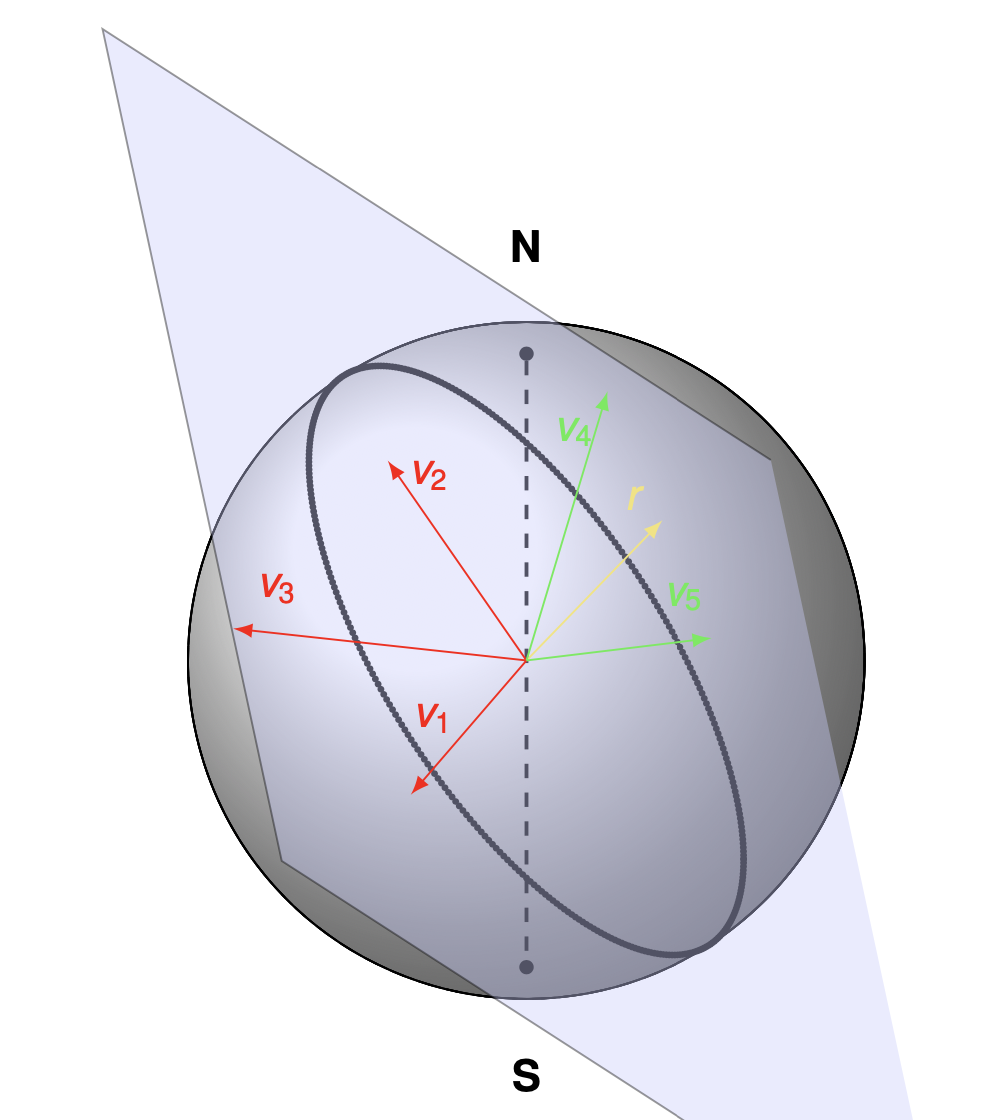
\includegraphics[scale=0.4]{5.png}
\end{figure}

\begin{lemma}
    Para cualquier $x \in [-1,1]$,
    \[
        \frac{1}{\pi} \arccos(x) \geq 0.878 \cdot \frac{1}{2}(1-x).
    \]
    \begin{figure}[H]
        \centering
            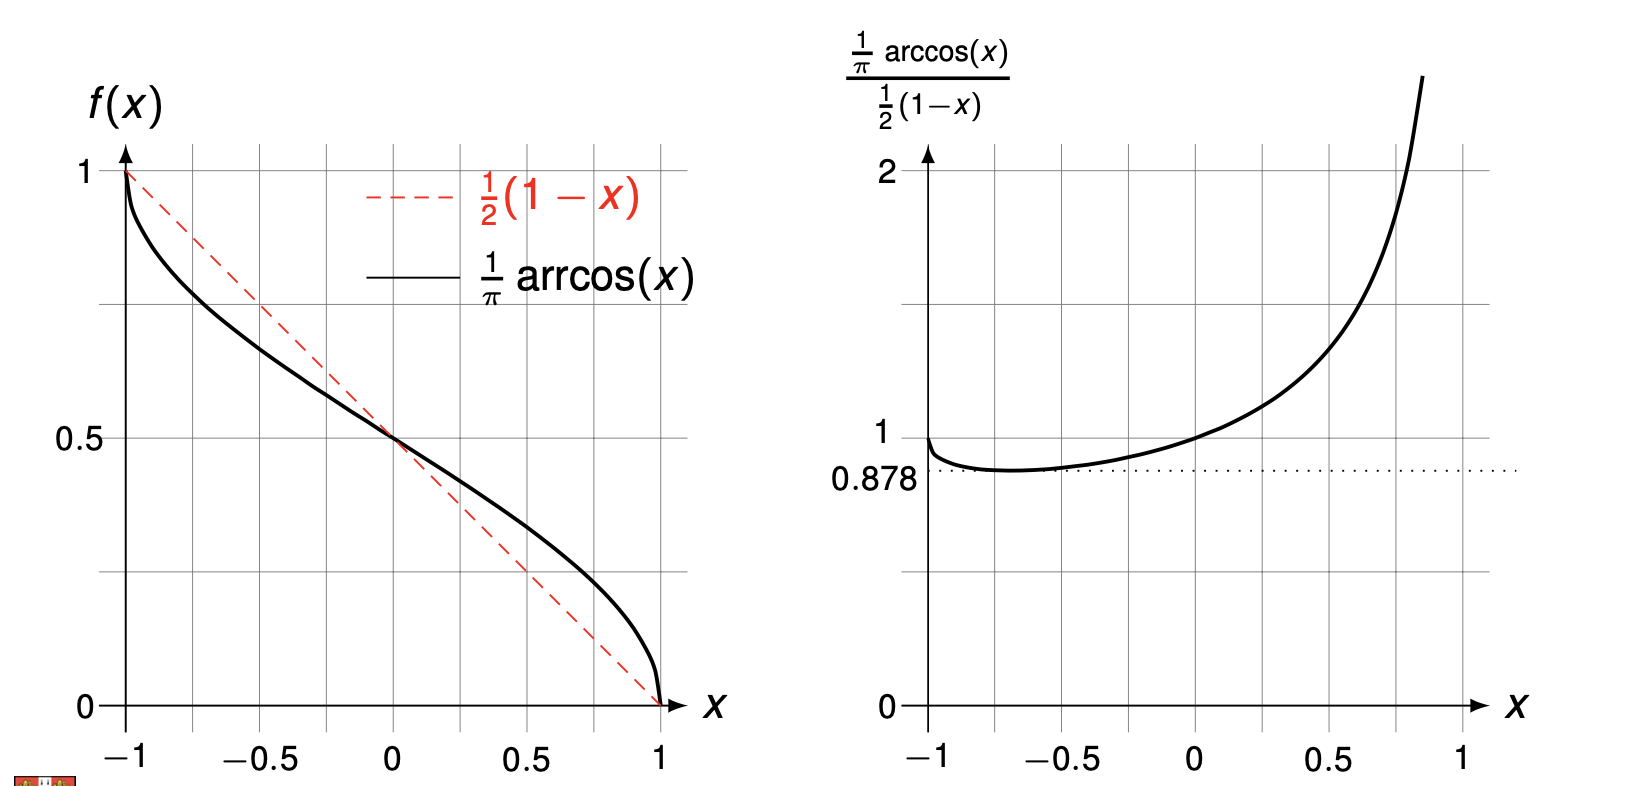
\includegraphics[scale=0.5]{6.png}
    \end{figure}
\end{lemma}

\begin{theorem}
    El algoritmo tiene una proporción de aproximación de $\frac{1}{0.878} \approx 1.139$. 
\end{theorem}

\section{$k$-Coloring}
Dada una gráfica simpe $G=(V,E)$ con un conjunto de vértives $V$ y un conjunto de aristas $E$, una
coloración de $G$ is una asignación de colores a cada vértives donde cada vértice adyacente tiene
diferentes colores. Una coloración óptimas de una gráfica arbitraria, i.e., el problema de determinar
el mínimo número de colores usaados para una gráfica arbitraria, es un problema NP-C bien conocido.
Aceptación por umbrales y búsqueda Tabú han sido adaptados para encontrar una $k$-coloración de una
gráfica dada  para un número fijo $k$.

Definimos el problema de la $k$-coloración más formalmente como sigue. Una partición de color de una
gráfica es una partición de su conjunto de vértices $V$ e subconjuntos llamados clases de colores,
$V = V_1 \cup V2 \cup \ldots \cup V_k$, donde los subconjuntos $V_i$ $(1 \geq i \geq k)$ son no vacíos
y mutamente disjuntos, y cada uno no contiene nungun par de vértices adyacentes.
El conjunto de las aristas ``malas'' $B$ estñas definido como
$B = \{ a \in E | a \in \cup_{i=1}^k V_i \times V_i \}$. Que es, el entero $|B|$ el número total de
aristas teniendo el mismo color en ambas de sus vértices incidentes. El conjunto de todas las
las aristas ``buenas'' es definido como $E \setminus B$. Definimos el problema de la $k$-coloración
como el problema de encontrar el número mñas grande de aristas ``buenas'' (o el número más pequeño
de aristas ``malas'') incidentes al conjunto de vértices el cual puede ser coloreado con $k$-colores
en una gráfica dada $G$.

Más formalmente, nos preguntamos por una partición de un conjunto de vértices $V$ en $k$ subconjuntos
$V_1, V_2, \ldots, V_k$ tal que:
\[
    \sum_{x\in \bigcup_{i=1}^{k} V_i \times V_i} weight(x)
\]
sea mínima. Observamos que el problema se convierte en el problema de maxcut cuando $k=2$.
\begin{algorithm}[H]
    \caption{Algoritmo $\mathcal{B}$: $k$-coloración}
    \hspace*{\algorithmicindent} \textbf{Input} $G=(V,E)$ \\
    \hspace*{\algorithmicindent} \textbf{Output} $k$ particiones $V_1,V_2,\ldots,V_k$ tal que el número de aristas ``malas'' en $G$ sea mínimo\\
    \begin{algorithmic}
    \STATE{ncut = 1; (* el número de cortes *)}
    \STATE{ncol = 0; (* el número de colores *)}
    \STATE{initqueue(Q); (* inicializa la cola $Q$ *)}
    \STATE{inqueue(Q, G); (* inserta $G$ en $Q$ *)}
    \WHILE{ncut $<$ k}
        \STATE{g = dequeue(Q); (* quita un elemento de $Q$ *)}
        \IF{$\exists$ aristas en $g$}
            \STATE{Simmax(g,a,b);}
            \STATE{ncut = ncut + 1;}
            \STATE{inqueue(Q, a);}
            \STATE{inqueue(Q, b);}
        \ELSE
            \STATE{ncol = ncol + 1;}
            \STATE{C[ncol] = g;}
            \ENDIF
            \ENDWHILE
    \WHILE{empty(Q) $\not=$ TRUE}
        \STATE{ncol = ncol + 1;}
        \STATE{C[ncol] = dequeue(Q);}
    \ENDWHILE
    \end{algorithmic}
\end{algorithm}

En esta sección, presentamos un tiempreo aproximado del algoritmos de $O((e+n)\log k)$ para colorear
una gráfica usando $k$-colores tal que el número de malas aristas no exceda $(e/k)((n-1)/n)^{\log k}$,
cuando $k = 2^h$ donde $h$ es un entero positivo. La cota es un poco menor que $e/k$. Por tanto,
nuestro algoritmo mejora tanto la cota $e/k$ y el tiempo de complejidad $O(enk)$ sabido antes cuando
$k = 2^h$. Se empleará una descomposición de arbol binaria para particionar la gráfica en dos
subgráficas recursivamente. En cada paso, generamos un corte máximo entre dos subgráficas usando nuestro
algoritmo Simmax propuesto. Las subgráficas obtenidas serán posteriormente particionadas hasta que tengamos
un total de $k = 2^h$ subgráficas. Notar que una subgráfica no será pasticionada si no continiene ninguna
arista mala. Podemos llamar al árbol binario generado un árbol de color corte máximo. Minimizando el
corte a cada nivel de arriba para abajo del color del árbol, el número de malas aristas será
gradualmente reducido. Ahora , basado en la construcción de la descomposición del árbol binario, una
implementación detallada del llamado $k$-coloración $(k-C)$ algoritmo es mostrada en el algoritmo de arriba.

Por tanto, podemos concluir que:

\begin{theorem}
    Existe un algoritmo en tiempo $O((e+n)\log k)$ para el problema de la $k$-coloración tal que el
    número totral de aristas en la $k(=2^h)$ subgráficas es a lo más
    $(e/k)((n-1)/n)^{\log k}$ (para el caso con pesos, $(w(E)/k)((n-1)/n)^{\log k}$), donde $h$ es la
    altura del árbol de color maxcut.
    \begin{proof}
        El número total de aristas en $V_1$ más el número total de aristas en $V_2$ son a lo más
        $|B_i| = e(G)(1-(n+1)/2n)=\frac{e(G)(n-1)}{2n}$.
        Por tanto en el nivel 2 del árbol de color maxcut, las subgráficas definidas por $V_1$ y $V_2$
        serán posteriormente divididas en $V_a$ y $V_b$, $V_c$ y $V_d$ respectivamente, y de nuevo tenemos:
        \[
            |B_2| = e(V_a) + e(V_b) + e(V_c) + e(V_d) \geq |B_1| (1 - (n+1)/2n) = e(G)(\frac{n-1}{2n})^2.
        \]
        Pariciones similares nos dan el número de malas aristas en el nivel $h = \log k$,
        \[
            |B_{\log k}| = e(V_1) + e(V_2) + \ldots + e(V_k) \geq e(G)(\frac{n-1}{2n})^{\log k} =
            \frac{e(G)}{k}(\frac{n-1}{2n})^{\log k}.
        \]
        
    \end{proof}
\end{theorem}

%%%%%%%%%%%%%%%%%%%%%%%%%%%%%%%%%%%%%%%%%%%%%%%%%%%%%%%%%%%%%%%%%%%%%%%%%%%%%%%%%%%%%%%%%

%%%%%%%%%%%%%%%%%%%%%%%%%%%%%%%%%%%%%%%%%%%%%%%%%%%%%%%%%%%%%%%%%%%%%%%%%%%%%%%%%%%%%%%%%



%%%%%%%%%%%%%%%%%%%%%%%%%%%%%%%%%%%%%%%%%%%%%%%%%%%%%%%%%%%%%%%%%%%%%%%%%%%%%%%%%%%%%%%%%
\nocite{*}


\bibliographystyle{plain}
\bibliography{references}
%%%%%%%%%%%%%%%%%%%%%%%%%%%%%%%%%%%%%%%%%%%%%%%%%%%%%%%%%%%%%%%%%%%%%%%%%%%%%%%%%%%%%%%%%

\end{document}